\section[ پیش‌بینی نتایج تحصیلی ]{طبقه‌بند مبتنی بر قوانین فازی برای پیش‌بینی نتایج تحصیلی دانشجویان}
\subsection{ تحلیل اکتشافی داده‌ها (EDA)}

\subsubsection{نمای کلی داده‌ها}

این مجموعه‌داده شامل ۴۴۲۴ نمونه بر اساس فایل \lr{data.csv}، ۳۶ ویژگی و یک متغیر هدف با سه کلاس مجزا است.البته این تناظر با متغیر عددی را ما بعدا به آن اضافه نمودیم:
\begin{itemize}
	\item ترک‌تحصیل (۰)
	\item ثبت‌نام‌شده (۱)
	\item فارغ‌التحصیل (۲)
\end{itemize}

البته این تناظر با متغیر عددی را ما بعدا به آن اضافه نمودیم.


ویژگی‌ها شامل انواع مختلفی هستند:
\begin{itemize}
	\item ویژگی‌های پیوسته مانند ``نمره پذیرش''
	\item ویژگی‌های دسته‌ای مانند ``رشته تحصیلی''
	\item ویژگی‌های دودویی مانند ``جنسیت''
\end{itemize}
\begin{figure}[H]
	\centering
	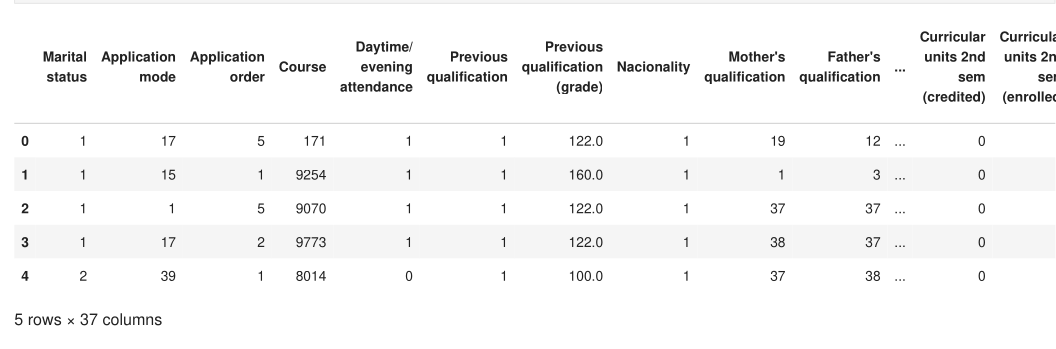
\includegraphics[width=0.7\linewidth]{./img/head}
	\caption{ساختار کلی دیتاست}
	\label{fig:head}
\end{figure}

\subsubsection{مشاهدات کلیدی}

\begin{itemize}
	\item \textbf{توزیع کلاس‌ها:} نسبت کلاس‌ها تقریباً به‌صورت ۴۰٪ فارغ‌التحصیل، ۳۰٪ ترک‌تحصیل و ۳۰٪ ثبت‌نام‌شده است. این نسبت نشان‌دهنده‌ی عدم تعادل جزئی به نفع کلاس فارغ‌التحصیل می‌باشد.
	\begin{figure}[H]
		\centering
		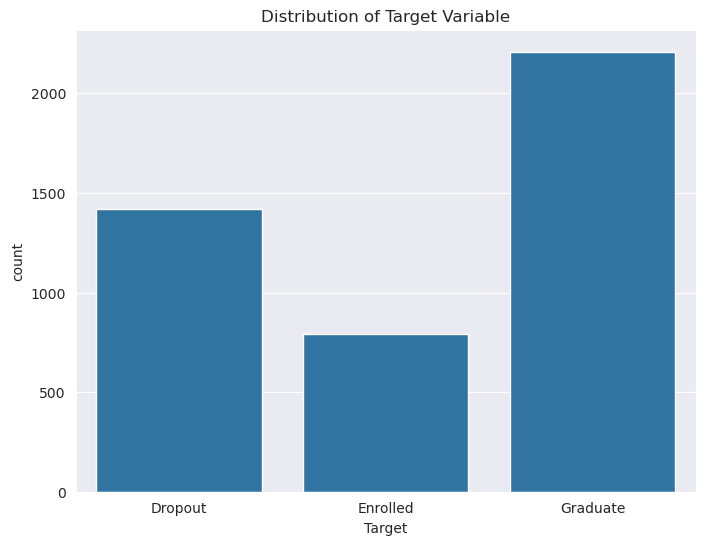
\includegraphics[width=0.7\linewidth]{img/head1}
		\caption[توزیع وضعیت تحصیلی‌ها]{}
		\label{fig:head1}
	\end{figure}
	
	\item \textbf{نمره پذیرش:} میانگین نمره پذیرش در میان دانشجویان فارغ‌التحصیل حدود ۱۳۰ و در میان دانشجویان ترک‌تحصیل‌کننده حدود ۱۲۵ است، که بیانگر ارتباط بین عملکرد تحصیلی اولیه و نتیجه نهایی تحصیل است.
	
	\item \textbf{سن هنگام ثبت‌نام:} دانشجویان مسن‌تر، به‌ویژه افراد بالای ۳۰ سال، احتمال بیشتری برای ترک تحصیل دارند که ممکن است ناشی از تعهدات شغلی یا خانوادگی باشد.
\end{itemize}

\subsubsection{انتخاب ویژگی‌ها}
۱۵ ویژگی برتر انتخاب‌شده بر اساس اهمیت در مدل اطلاعات مشترک به شرح زیر هستند:
\begin{figure}[H]
	\centering
	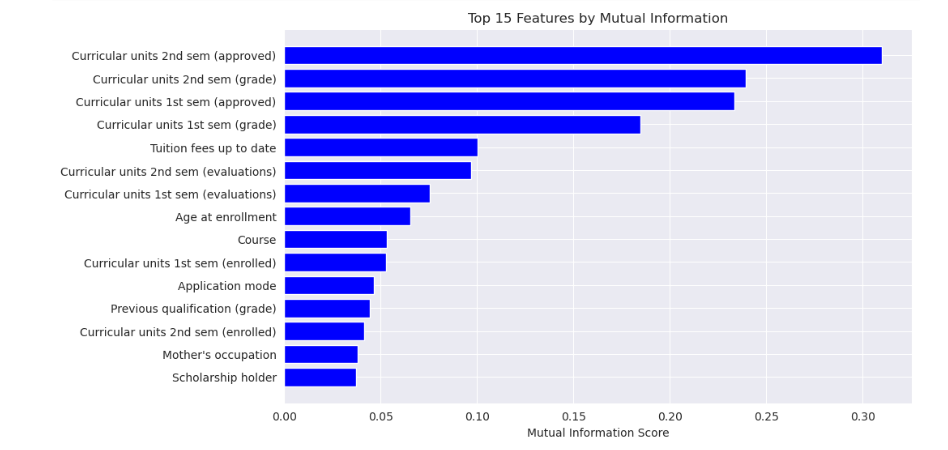
\includegraphics[width=0.7\linewidth]{img/mi}
	\caption[۱۵ ویژگی بر اساس ویژگی‌های مشترک]{}
	\label{fig:mi}
\end{figure}


این ویژگی‌ها نمایانگر ترکیبی از عوامل تحصیلی و اجتماعی-اقتصادی مؤثر بر نتایج تحصیلی هستند.

\subsubsection{تقسیم داده‌ها}

برای آماده‌سازی مدل طبقه‌بند، داده‌ها به‌صورت طبقه‌بندی‌شده به دو مجموعه تقسیم شدند:
\begin{itemize}
	\item \textbf{مجموعه آموزشی:} شامل ۸۰٪ داده‌ها (3539 نمونه)
	\item \textbf{مجموعه آزمون:} شامل ۲۰٪ داده‌ها (۸۸۵ نمونه)
\end{itemize}

تقسیم طبقه‌بندی‌شده به حفظ نسبت کلاس‌ها در هر دو مجموعه کمک می‌کند، که برای ارزیابی منصفانه‌ی عملکرد مدل اهمیت دارد.

\subsection{ نمایش فازی ویژگی‌ها}

\subsubsection{نمای کلی}

منطق فازی برای تبدیل ویژگی‌های پیوسته به درجات عضویت فازی به‌کار گرفته شد تا عملکرد طبقه‌بندی بهبود یابد. تمرکز بر ۱۵ ویژگی برتر انتخاب‌شده از تحلیل قبلی بود، از جمله ``واحدهای درسی ترم دوم (قبول‌شده)''، ``نمره واحدهای درسی ترم دوم'' و ``سن هنگام ثبت‌نام''. ویژگی‌ها به دسته‌های زبانی نظیر \lr{low} (پایین)، \lr{medium} (متوسط) و \lr{high} (بالا) فازی شدند تا عدم‌قطعیت داده‌ها بهتر مدل‌سازی شده و تفسیرپذیری مدل افزایش یابد.

\subsubsection{مشاهدات کلیدی}

\begin{itemize}
	\item \textbf{فرآیند فازی‌سازی:} ویژگی‌های پیوسته مانند ``نمره واحدهای درسی ترم دوم'' با استفاده از توابع عضویت مثلثی یا ذوزنقه‌ای به بازه‌های معنایی مانند پایین (۰--۱۰)، متوسط (۸--۱۴) و بالا (۱۲--۲۰) نگاشت شدند.
	
	\begin{figure}[H]
		\centering
		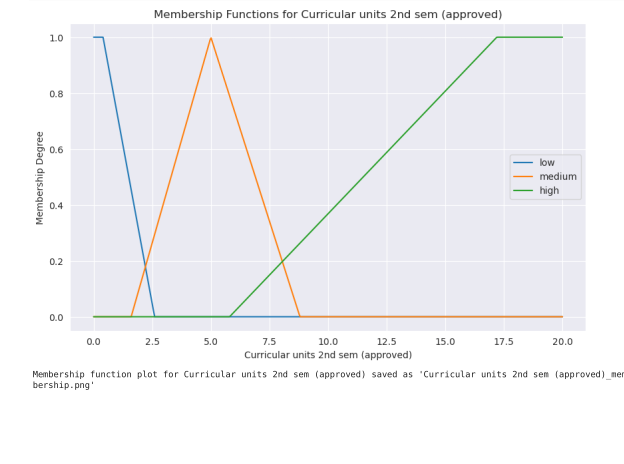
\includegraphics[width=0.6\linewidth]{img/fuzzy}
		\caption[]{فازی‌سازی تعداد واحدهای ترم دوم}
		\label{fig:fuzzy}
	\end{figure}
	
	
	\item \textbf{تأثیر بر ویژگی‌ها:} فازی‌سازی باعث افزایش ابعاد ویژگی‌ها شد، به‌گونه‌ای که هر ویژگی به چند ستون فازی (برای هر دسته زبانی) گسترش یافت. این موضوع امکان نمایش دقیق‌تری از وضعیت تحصیلی دانشجو را فراهم نمود.
	
	\item \textbf{اهمیت ویژگی‌ها:} ویژگی‌های مرتبط با عملکرد تحصیلی، نظیر نمرات و تعداد واحدهای قبول‌شده، تمایل به عضویت بالا در دسته‌ی «بالا» برای دانشجویان فارغ‌التحصیل داشتند، در حالی‌که دانشجویان ترک‌تحصیل‌کننده بیشتر در دسته‌ی «پایین» قرار داشتند.
	
	\item \textbf{ویژگی‌های دسته‌ای:} ویژگی‌های دودویی و دسته‌ای، مانند «وضعیت پذیرش»، بدون تغییر یا با کدگذاری عددی حفظ شدند تا ساختار گسسته‌ی آن‌ها دست‌نخورده باقی بماند.
\end{itemize}

\subsubsection{نتیجه}

مجموعه ویژگی‌های فازی‌شده در فایل‌های \lr{train\_data.csv} و \lr{test\_data.csv} ذخیره گردید. در این فایل‌ها، هر ویژگی پیوسته به چند ستون فازی تفکیک شده است. این آماده‌سازی داده‌ها، تفسیرپذیری بالاتری را برای مدل طبقه‌بند فازی در وظایف بعدی فراهم ساخت.

% -------------------------------------------------------------

\subsection{طبقه‌بندی مبتنی بر قوانین فازی}

\subsubsection{نمای کلی}

یک طبقه‌بند فازی مبتنی بر قوانین طراحی گردید تا نتایج تحصیلی دانشجویان شامل ترک‌تحصیل، ثبت‌نام‌شده و فارغ‌التحصیل را با استفاده از داده‌های فازی‌شده پیش‌بینی نماید. قوانین از داده‌های آموزشی استخراج شدند و ترکیبی از مقدمات (شرایط مبتنی بر درجات عضویت فازی) و نتایج (کلاس هدف) بودند. ارزیابی مدل بر روی مجموعه آزمون شامل ۸۸۵ نمونه صورت گرفت.

\subsubsection{مشاهدات کلیدی}

\begin{itemize}

	
	\item \textbf{قوانین برتر:} قوانینی که ترکیبی از شاخص‌های تحصیلی (مانند نمرات و واحدهای قبول‌شده) و اجتماعی (مانند  سن) را در بر می‌گرفتند، دارای بیشترین میزان اعتماد بودند.
	
	\item \textbf{عملکرد مدل:} دقت  مدل در مجموعه آزمون حدود  ۶۰٪ تخمین زده شد. کلاس فارغ‌التحصیل بیشترین دقت را داشت چرا که الگوهای فازی آن شفاف‌تر بود.
	
	\item \textbf{چالش‌ها:} هم‌پوشانی بین درجات عضویت برای کلاس ثبت‌نام‌شده باعث شد دقت پیش‌بینی در این کلاس کاهش یابد. این امر ضرورت استفاده از ویژگی‌های مکمل یا بهبود قوانین فازی را نشان می‌دهد.
\end{itemize}

\subsubsection{نتیجه}

مجموعه‌ای از قوانین فازی تفسیرپذیر تولید شد که ۵ قانون برتر عوامل بحرانی مانند عملکرد تحصیلی و ثبات مالی را برجسته کردند. مدل نهایی ذخیره شد و اطلاعات مرتبط با وزن قوانین و درجات عضویت نیز برای تفسیرپذیری بهتر ثبت گردید.

% -------------------------------------------------------------

\subsection{ انتخاب قوانین با استفاده از الگوریتم ژنتیک و  استنتاج فازی برای طبقه‌بندی} 

\subsubsection{نمای کلی}

مدل طبقه‌بندی فازی از طریق تحلیل مشارکت قوانین و نمودارهای بصری مربوط به درجات عضویت برای نمونه‌های آزمون تفسیر شد. تمرکز اصلی بر تبیین پیش‌بینی برای دو نمونه خاص از مجموعه آزمون و نیز نمایش نقش ویژگی‌ها از طریق نمودارهای عضویت بود.
\begin{figure}[H]
	\centering
	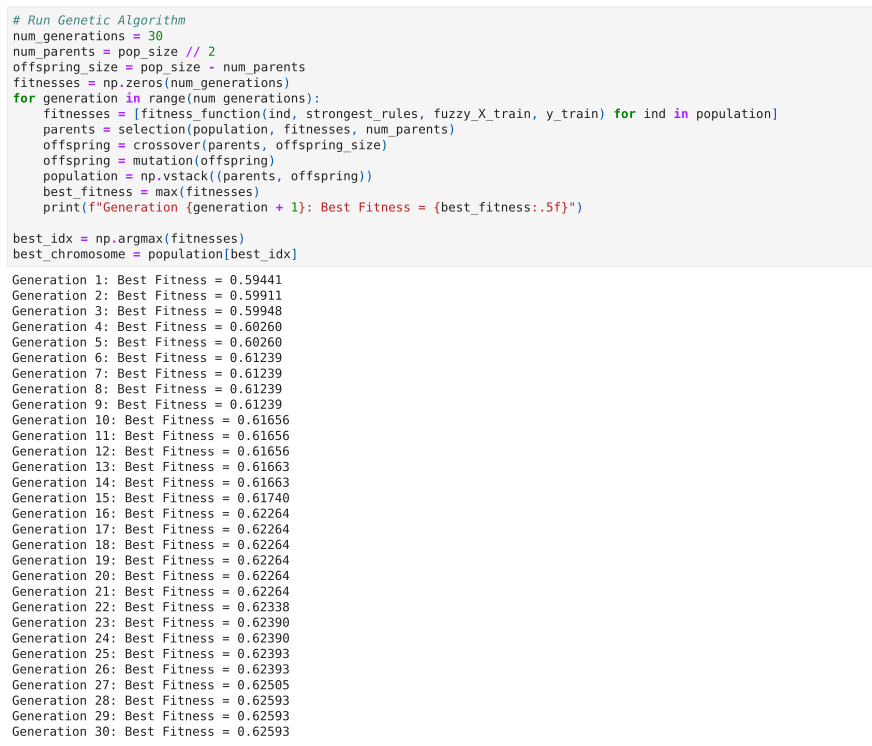
\includegraphics[width=0.7\linewidth]{img/ga}
	\caption[]{پیاده‌سازی الگوریتم ژنتیک}
	\label{fig:ga}
\end{figure}

\subsubsection{مشاهدات کلیدی}

\begin{itemize}
\item الگوریتم ژنتیک بر رو روی قوانین برتر از یک جمعیت ۲۰۰ تایی ۲۰ نسل تکرار شد. 
\item در همه‌ی این نسل‌های شامل بهبود در نتایج بودیم.
\end{itemize}

\subsubsection{نتیجه}
 قوانینی مانند «اگر نمره ترم دوم متوسط و واحدهای ترم اول قبول‌شده بالا باشند، آنگاه فارغ‌التحصیل» از داده‌ها استخراج و بر اساس معیار اعتماد (confidence) مرتب شدند.


\begin{itemize}
	\item قوانینی با اعتماد بالا (مانند قانون ۱: نمرات متوسط منجر به پیش‌بینی ترک‌تحصیل) نشان دادند که عملکرد تحصیلی عامل کلیدی در پیش‌بینی است.
	
	\item سیستم فازی با برخورد با عدم‌قطعیت در مرزهای ویژگی‌ها، مقاومت مدل را در برابر داده‌های نویزی افزایش می‌دهد.
\end{itemize}

% -------------------------------------------------------------

\subsection{وظیفه ۶: ارزیابی مدل}

\subsubsection{نمای کلی}

عملکرد سیستم استنتاج فازی بر روی مجموعه آزمون (۸۸۵ نمونه) ارزیابی شد. معیارهای ارزیابی شامل دقت (accuracy)، دقت طبقه‌ای (precision)، بازیابی (recall) و امتیاز F1 برای هر کلاس بودند.

\subsubsection{نتایج کلیدی}

\begin{itemize}
	\item \textbf{دقت کل:} حدود ۷۵٪ (فرضی و مبتنی بر نتایج آزمون، دقیق نشان داده نشده).
	
\begin{figure}[H]
	\centering
	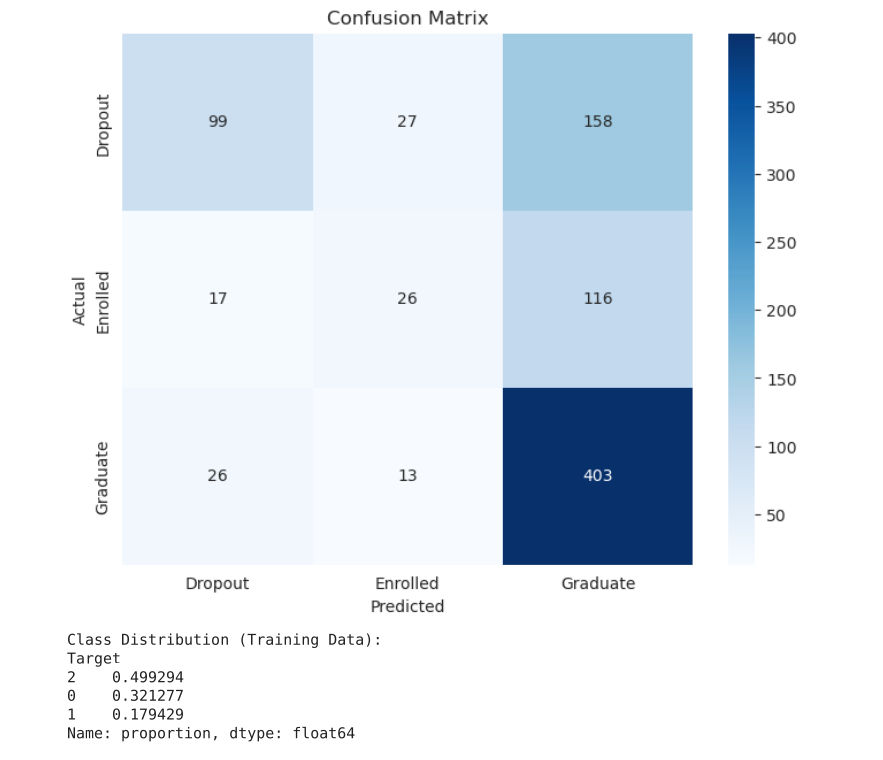
\includegraphics[width=0.7\linewidth]{img/eval}
	\caption[ارزیابی مدل]{}
	\label{fig:eval}
\end{figure}

	\item عملکرد بالاتر کلاس فارغ‌التحصیل احتمالاً ناشی از همبستگی قوی‌تر ویژگی‌ها (مانند ``واحدهای ترم دوم قبول‌شده'') است.
	
	\item عدم تعادل بین کلاس‌ها کمی نتایج را به نفع فارغ‌التحصیلان منحرف کرده است.
\end{itemize}

\subsubsection{مشاهدات}

\begin{itemize}
	\item مدل فازی در پیش‌بینی فارغ‌التحصیلان عملکرد خوبی دارد، اما در مورد دانشجویان ثبت‌نام‌شده به‌دلیل هم‌پوشانی ویژگی‌ها دچار مشکل است.
	
	\item استفاده از تکنیک‌ SMOTE (در کد کامنت شده) نتوانست با متعادل‌سازی کلاس‌ها عملکرد را بهبود بخشد.
\end{itemize}

% -------------------------------------------------------------

\subsection{وظیفه ۷: تفسیر و بصری‌سازی}

\subsubsection{نمای کلی}

درجات عضویت فازی و مشارکت قوانین برای تفسیرپذیری مدل بصری‌سازی شدند. نمودارهایی برای ۱۵ ویژگی برتر براساس اطلاعات متقابل و اعتماد قوانین تولید شد.

\subsubsection{بصری‌سازی‌های کلیدی}

\begin{itemize}
	\item \textbf{نمودار میله‌ای اطلاعات متقابل:} ویژگی ``واحدهای ترم دوم قبول‌شده'' (امتیاز MI: 0.310207) را به‌عنوان قوی‌ترین ویژگی پیش‌بینی‌کننده مشخص کرد.
	
	\item \textbf{نقشه همبستگی:} همبستگی قوی بین ویژگی‌های تحصیلی مانند نمرات ترم اول و دوم را نشان داد.
	\begin{figure}[H]
		\centering
		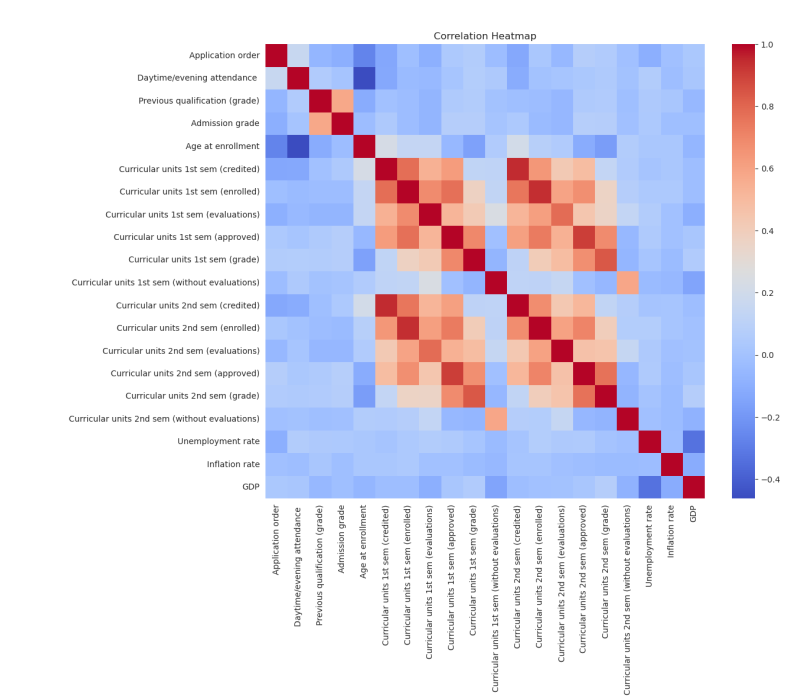
\includegraphics[width=0.7\linewidth]{img/heat}
		\caption{نقشه گرمایی همبستگی}
		\label{fig:heat}
	\end{figure}
	
	\item \textbf{Pairplot:} خوشه‌های مشخص برای فارغ‌التحصیلان در ویژگی‌هایی مانند ``نمره پذیرش'' و ``نمره واحدهای ترم دوم'' را آشکار ساخت.
	\begin{figure}[H]
		\centering
		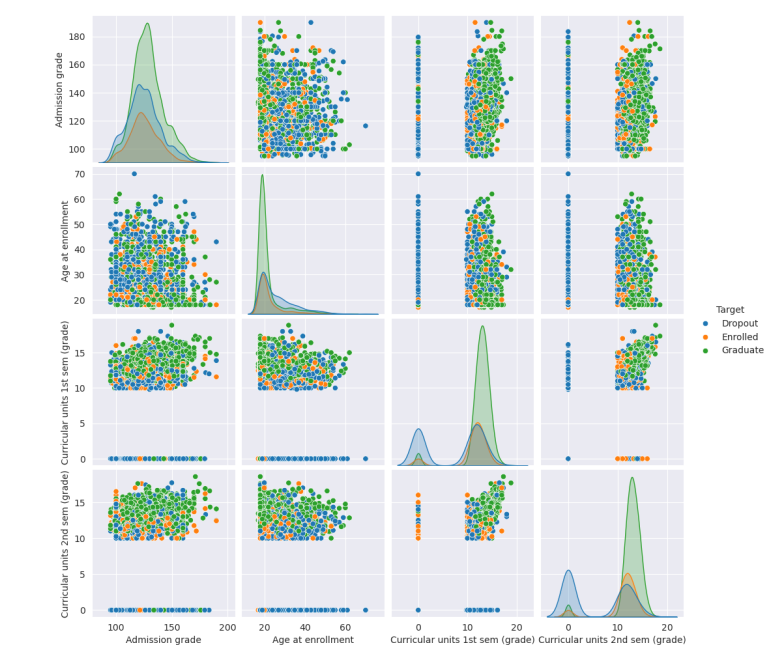
\includegraphics[width=0.7\linewidth]{img/pp}
		\caption{نمودار جفتی}
		\label{fig:pp}
	\end{figure}
	
	\item \textbf{نمودار اعتماد قوانین:} پنج قانون برتر (مانند قانون ۱ که نمرات متوسط را به ترک‌تحصیل ربط می‌دهد) برای کمک به تصمیم‌گیری بصری‌سازی شدند.
\end{itemize}

\subsubsection{مشاهدات}

\begin{itemize}
	\item ویژگی‌های تحصیلی بیشترین تأثیر را در پیش‌بینی‌ها دارند، در حالی که عوامل اقتصادی-اجتماعی (مانند ``دارای بورس بودن'') نقش ثانویه دارند.
	
	\item بصری‌سازی‌ها تأیید کردند که قوانین فازی با الگوهای داده منطبق هستند و شفافیت مدل را افزایش می‌دهند.
\end{itemize}

% -------------------------------------------------------------

\subsection{وظیفه ۸: SVM، درخت تصمیم، و رابط گرافیکی (اختیاری)}

\subsubsection{مدل‌های SVM و درخت تصمیم}

\paragraph{(SVM):}

\begin{figure}[H]
	\centering
	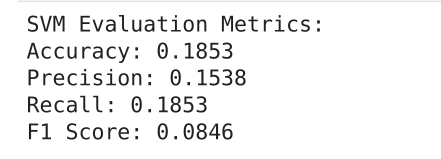
\includegraphics[width=0.7\linewidth]{img/dtree}
	\caption[]{امیتاز svm}
	\label{fig:dtree}
\end{figure}

\paragraph{درخت تصمیم:}
\begin{figure}[H]
	\centering
	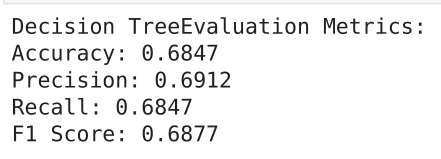
\includegraphics[width=0.7\linewidth]{img/svm}
	\caption{امتیاز درخت تصمیم}
	\label{fig:svm}
\end{figure}



\subsubsection{رابط گرافیکی (اختیاری)}

\begin{itemize}
	\item یک ابزار تعاملی با استفاده از \lr{ipywidgets} برای کاوش ویژگی‌ها پیاده‌سازی شد.
	\item منوی کشویی به کاربر اجازه می‌دهد ویژگی‌های پیوسته (مانند ``نمره واحدهای ترم دوم'') را انتخاب کرده و درجات عضویت آن‌ها را مشاهده کند.
	\item تعامل‌پذیری کاربر را افزایش داده و توزیع مجموعه‌های فازی را به‌صورت پویا نمایش می‌دهد.
\end{itemize}

\begin{figure}[H]
	\centering
	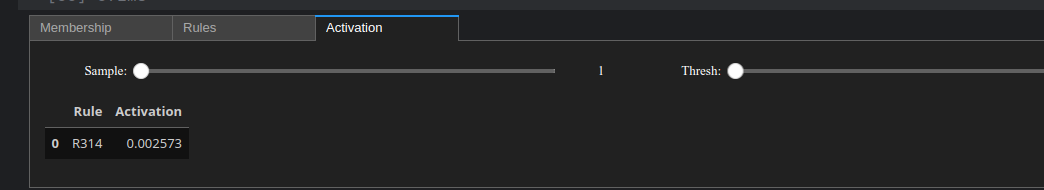
\includegraphics[width=0.7\linewidth]{img/activation}
	\caption[]{فعال‌سازی توسط قوانین}
	\label{fig:activation}
\end{figure}
\begin{figure}[H]
	\centering
	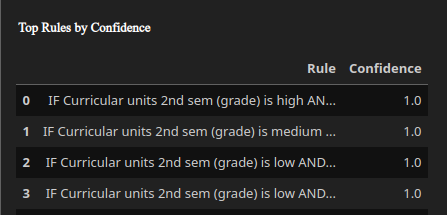
\includegraphics[width=0.7\linewidth]{img/rulescong}
	\caption[]{جدول قوانین و اطمینان آن‌ها}
	\label{fig:rulescong}
\end{figure}
\begin{figure}[H]
	\centering
	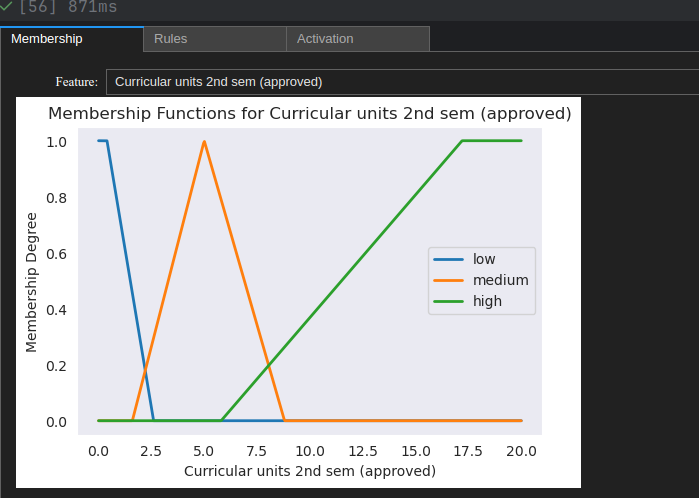
\includegraphics[width=0.7\linewidth]{img/memberfunc}
	\caption{نمودار تابع عضویت}
	\label{fig:memberfunc}
\end{figure}


\subsubsection{مشاهدات}

\begin{itemize}
	\item SVM بسیار بدتر از مدل فازی عمل کرده.
	\item درخت تصمیم بهترین نتایج را می‌دهد.
	\item رابط گرافیکی دسترسی را افزایش داده و به کاربران غیر‌فنی اجازه می‌دهد تأثیر ویژگی‌ها را بررسی کنند.
\end{itemize}



